\chapter{Analysis}
\label{chap:analysis}

The debugging activity collected 6890 snapshots over 119 projects. The temperature activity collected 2296 snapshots over 35 projects. In total, 9186 snapshots were analyzed. From these data, features were extracted that represented the type of code change that occurred in a snapshot. After some analysis of these change-type features, a new analytical method was constructed to provide teachers with useful information towards identifying flailing, off-task, or disengaged behavior. The new method, called \emph{solution particle analysis,} did not depend on the change-type features, instead using purpose-specific new feature extractor. This technique is described below in Section \ref{sec:particle-analysis}.

The particle analysis method allowed for the development of a visual display tool that allowed immediate insight into the state of a classroom in the recorded data, in such a way that would aid a teacher in coordinate their resources. 

The process of generating the extracted features, which served as the raw data for all analysis techniques, is discussed below in Section \ref{sec:data-processing}.


\section{Data Processing Pipeline}
\label{sec:data-processing}
% Data Pipeline:
% filter to relevant projects in database ->
% processProject:
%	load change contents from git
%		fix trailing xml corruption
%		checks for empty blocks, only includes if not-empty
%		generate IDmaps and parentmaps
%	extract changes
%		check for:
%			added/Deleted blocks
%			movedblocks
%			contextMove
%			changedblocks
%			fieldchanges
% 	reduceFieldChanges
%	generateChangeIntervals

Data was imported from the git database into the analysis environment using a process shown in Figure \ref{fig:data-import-process}. The key step of this process was ``Extract change features,'' where the tests for the types of changes in that snapshot were executed. Feature extraction is described in detail below in Section \ref{sec:feature-extraction}.

\begin{figure}
  \centering
      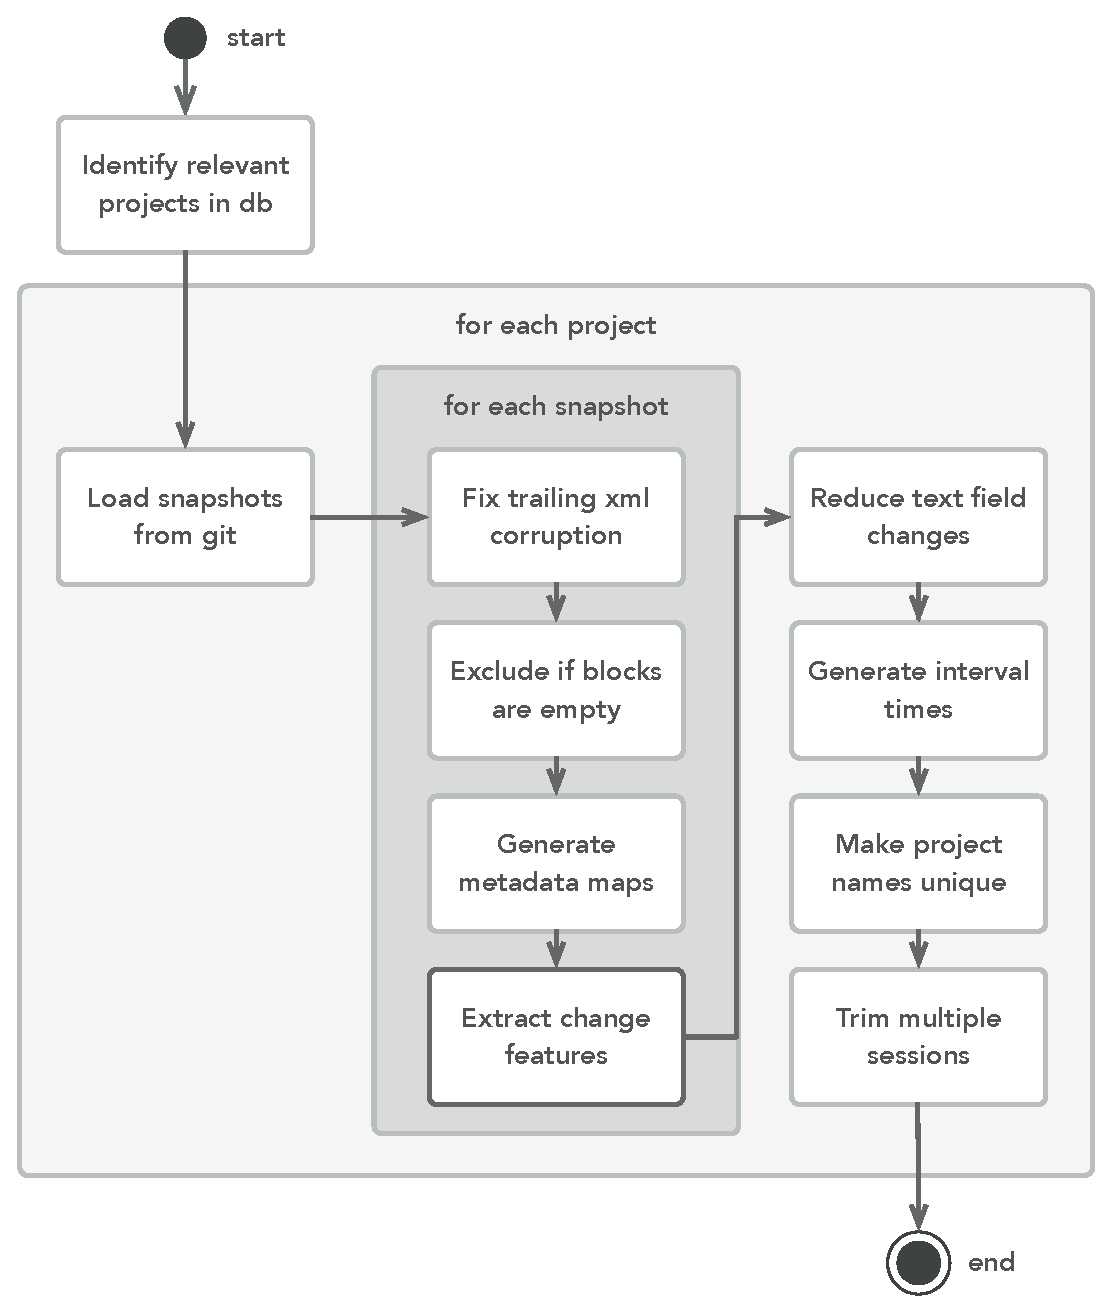
\includegraphics[width=\textwidth]{diagrams/data-import-process}
  \caption[The data importing process]{The data importing process. The entire database was scanned for projects that contain an identifiable element, which were then loaded directly from git. Each change from git was processed for error mitigation and necessary metadata generation, then the features were extracted. After feature extraction, character-wise text field changes were reduced, and then the interval times between snapshots were generated.}
  \label{fig:data-import-process}
\end{figure}

The import pipeline had many tasks to accomplish, starting with identifying the projects that were relevant for analysis. The App Inventor instance that was used for this study was also used for the entirety of the summer camp curricula, so there were many projects captured in the snapshot database that were not part of the activities specific to this study. This was an intentional part of the protocol to make transition easier for the camp students by only having one App Inventor instance with which to interface. The in-class activities were better isolated, so researchers were able to prepare the room in advance to steer the students transparently towards the specialized instance. 

The activities that were part of this study needed to be found in the database. Students had the ability to rename projects at any point, so it was possible (albeit unlikely) that a relevant project could be renamed. Therefore the protocol included a unique element in the projects, a ``magic string'' in a hard-to-find property of the project. The debugging activity and temperature activity each had a unique identifier string, and these strings were included in the starter code that all students were given. These unique elements were then detectable by scanning the files in the git database prior to import. There were instances of students changing the names of the projects, which demonstrated the need of the unique identifier. 

Once a list of projects were identified using their unique elements, those projects were loaded from git into the analysis environment. The git interface opened each project's repository, extracted a list of all commits, and then checked out each commit in turn, capturing the contents of the files for each commit. A commit represented a single snapshot, and the terms ``snapshot'' and ``change'' were used interchangeably to describe the contents of the commit after this stage. 

Each snapshot was checked for corruption at time of import. Following that, two metadata maps were generated for each snapshot: a map of block ID numbers, and a map of block parents. These maps allowed the feature extractor to easily access a block by its ID number (which would require a full tree traversal without), and easily look up the parent of any given block. With the maps generated, the feature extractor would then be able to run. 

After feature extraction, the text field events were reduced (described below), and finally, with the snapshot set complete, interval times between snapshots were generated.

Most stages of the import process were additive and non-destructive, so at the conclusion of import each project and snapshot had all of the data available at all previous steps. For instance, the raw block contents were not lost during feature extraction; the list of features were added to the data structure alongside it. 

The following sections delve further into certain components of the import pipeline, and are presented in pipeline order: corruption mitigation, feature extraction, and text field reduction.


\subsection{Corruption Detection and Mitigation}
Some forms of corruption were found in the snapshot data, all concerning the blocks representation. There were four corruption modes, which are explained below, with their respective mitigation strategies.

The first corruption mode was malformed XML files which contained text beyond the closing XML tag. This, of course, crashed the XML parser. Within the debugging activities, only seven snapshots had this malformation, which were corrected by trimming the excess text. It was noteworthy in those cases that the junk excess text was a repetition of the last characters of the file, lends to a hypothesis of the source of the corruption, discussed below.

The second form was rare, where a snapshot had no contents for the blocks file. In the entire collection of debugging activity snapshots ($n = 6890$), only three snapshots had empty blocks. These snapshots were detected during import and were not included in the research data. The overall history of the projects containing these empty shapshots were unaffected. 

Both of these corruptions were indicative of a bug in the extraction of the block data from blockly in the browser. It was possible that the snapshot mechanism was able to capture the XML file while it was in an inconsistent state, such as mid-write. This bug may be within the Blockly framework itself, and further investigation is recommended before attempting larger-scale deployment of this method.

The two above corruptions were easily mitigated. A third mode of corruption, however, resulted in properly formed XML, but potentially erroneous data. This mode was characterized by multiple changes happening in a single snapshot, which should have been extremely rare, as each snapshot was triggered by an atomic action in the editor. In reality, there was a small amount of caching in the capture mechanism, as discussed in Section \ref{sec:mod-ai}, which may have contributed to this corruption. There was no inherent problem with multiple changes in a single snapshot, if they all occured within the capture window of that snapshot. In these erroneous cases, one or more actions appeared to be inconsistently represented over time, which caused git and the subsequent analysis tools to do, un-do, and re-do the same action in very small spans of time, artificially inflating the representation of those events. 

One project was particularly egregious, and showed this corruption in 71 of its 245 commits, rendering nearly a third of its data unreliable. That project was removed, which left only 50 such potential errors in the remainder of the database, many of which were mitigated by text field accumulator, described in Section \ref{sec:text-acc}. 

A data consistency bug was found where a project was opened over more than one session. In App Inventor, if a project was opened in a second, disjoint session, such as the following day, the block ID numbers change, causing the feature extractors to falsely over-report blocks being deleted and added, when really the same blocks have been re-numbered. The strategy employed was to ignore snapshots that occurred at a timestamp beyond the maximum time of the activity.

The total percentage of potentially erroneous snapshots in the debugging activity dataset was 0.84\%. These are summarized in Table \ref{tab:data-corruption}.

% % Debug:		empty blocks - 3 (now, many were hand-fixed, notes may indicate more)
% %				junk past tag - 7 (now, many were hand-fixed, notes may indicate more)
% %			6890 snapshots total
% % Temperature:	empty blocks - 1 
% %				junk past tag - 4 
% %			2296 snapshots total
	
\begin{table}
\begin{centering}
	\begin{tabular}{l r l p{5.4cm}}
	Corruption Mode 		& \multicolumn{2}{l}{Instance Count} 		& Mitigation Strategy 			\\ \hline
	Empty block file 						&  3 &(0.04\%) 				& snapshot deleted 						\\
	Junk beyond \mintinline{xml}|</xml>| 	&  7 &(0.1\%) 				& junk trimmed, snapshot kept 			\\
	Multiple changes 						& 50 &(0.7\%) 				& accepted as insignificant 			\\
	Multi-session 							&  3 &(0.04\%) 				& data past 40 minutes ignored
	\end{tabular}
	\caption[Data corruption modes]{Data corruption modes, their prevalence, and mitigation strategy.}
	\label{tab:data-corruption}
\end{centering}
\end{table}


\subsection{Feature Extractor}
\label{sec:feature-extraction}

\begin{table}
\begin{labeling}{Blocks Moved in Context}

	\item [Blocks Added] Block(s) were added to the workspace. Nearly always a single block.
	\item [Blocks Deleted] Block(s) were removed from the workspace.
	\item [Blocks Moved in Space] Block(s) moved position on the workspace, but did not necessarily change programmatic meaning.
	\item [Blocks Moved in Context] Block(s) changed programmatic position, indicating a new parent block and a different place in the app's control flow.
	\item [Fields Changed] A block's text field changed. Could be a text literal, a variable or procedure name, or a number literal.
	\item [Properties Modified] One or more properties of a block has changed, which could indicate use of the mutator to change a block's semantics (such as changing the number of addends in an addition block). Intended as a catch-all if the other tests missed something, and was rarely found in the data.
	
\end{labeling}
\caption[Features extracted from snapshots]{Features extracted from snapshot data.}
\label{tab:features-extracted}
\end{table}

The features extracted by this module were listed and described above in Figure \ref{tab:features-extracted}. This section outlines the specific definitions that constitute the feature tests. All of these tests operated on snapshots of the same project that were adjacent in time. They detected differences between the two, often utilizing the metadata maps described above in Section \ref{sec:data-processing}. Source code for these algorithms are presented in Appendix \ref{src:feature-extraction-tests}.

The test for \emph{Blocks Added} and \emph{Blocks Deleted} were the same routine, which assembled a list of blocks by their ID numbers for both snapshots and compared differences between those lists using set arithmetic. 

The test for \emph{Blocks Moved in Space} assembled a list of blocks that were present in both snapshots, and iterated that list looking for blocks who were both top-level and whose coordinates changed. There was an important distinction made here- blocks that were nested within other blocks were not top-level and therefore did not trigger the \emph{Blocks Moved in Space} flag when they moved as a consequence of their parent moving. Only blocks whose parent is the workspace itself may return positive from this test, and then, only if they actually moved on the workspace.

\emph{Blocks Moved in Context} was the opposite of the above test, where it detected if a block moved in computational context, indicated by a changed parent. Similarly, this test assembled a list of blocks common to both snapshots, and iterated across that list. The iteration checked if the parent for the block was the same in both snapshots, and returned true if they were not. 

To detect \emph{Fields Changed}, common blocks were listed and then filtered for field properties. Those fields were searched for cases where the value of the fields differed between the two snapshots.

The final test, \emph{Properties Modified} caught any other modifications to a block. This test was more complex. Like those above, it assembled a list of blocks present in both snapshots. It then ran an exhaustive element-wise equality check on each block, comparing the version in each snapshot. If the equality check returned true, that block did not change in any way. If the equality check was false, then lists of all children for both blocks were assembled, which included properties, data fields, mutator instructions, and other Blockly metadata. This step excluded text fields, as they were covered in a previous test. If the lengths of the lists of children were unequal, then the routine returned true, as these particular blocks definitely changed between the two snapshots. If they have the same number of children, then each pair of children were iterated, and the element-wise equal was applied to each of them, effectively running a first-level recursive equality test. If that test did not find any differences, then the routine returned false. That final false return is a condition that should be impossible, but was included defensively, as there may have been edge cases possible in Blockly that were not common in known to the researchers at the time of this design.


\subsection{Text Field Change Accumulator}
\label{sec:text-acc}
In the course of working on their activities, students often manipulated fields of text, including text literals, variable names, procedure names, and parameter names. Examples of blocks utilizing open text fields are shown in Figure \ref{fig:text-fields}. Whenever a text field was modified, the change event was triggered for every character. This was a degree of granularity too fine for meaningful analysis, as character modification events are considered too primitive to be of use \citep{omori2008change}. The snapshot system at runtime could not discern the beginning and end of field editing events, so the change event feature \emph{Fields Changed} from Table \ref{tab:features-extracted} was grossly over-represented. 

To combat this over-representation, sequences of character-wise change events needed to reduced to their final state, which then represented a single change at the same degree of abstraction as the surrounding block manipulations. This reduction was accomplished with an accumulator algorithm, which scanned a project's change history and identified uninterrupted sequences of field modifications to the same field. The algorithm deleted all but the final \emph{Fields Changed} events, leaving only the final state of the modification for further processing. This algorithm had a 10-second timeout, so sequential edits to the same field would be considered different events if there were more than 10 seconds between them. Changes to different field blocks were also considered a new event. This algorithm is shown and further explained in Appendix \ref{src:reduceFieldChanges}.

\begin{figure}
  \centering
      \includegraphics[width=\textwidth]{images/ch4-text-fields}
  \caption[Examples of text fields in App Inventor]{Examples of some text fields in App Inventor. All of the fields, represented by the text in shaded bubbles, could be edited arbitrarily by the student.}
  \label{fig:text-fields}
\end{figure}



\section{The Particle Analysis Method}
\label{sec:particle-analysis}

The purpose of this study was to develop a tool, informed by students' fine-grained programming activities, that can aid a teacher in deciding how to apply their resources during a lab session in real time. A significant insight was reached during analysis of the above change-type features, that such a tool could be constrained to standardized, ``on-rails'' programming assignments. These closed-ended assignments constitute the bulk of many curricula in use, such as those described by  \citet{gray2012teaching}, \citet{martin2015dual}, and \citet{morelli2015analyzing}, and are particularly common at the beginning of curricula, when students are still learning the basics. This situation would be the ideal use case for an orchestration aid. 

With this insight, and the constraint it brought, design began for both a visual tool to help a teacher orchestrate, and an analysis method to power it. The resulting method was \emph{particle analysis,} which borrowed its name from the behavior of atoms and molecules. With this method, a solution to an activity can be regarded as a complex molecule, which was built up out of smaller molecules, which were themselves composed of atoms. In this analogy, every individual block was an atom, and were combined on the workspace to make expressions, representing molecules. A solution to an activity was one or more of these molecules, which could have any number of atoms within them. The analogy could be further extended, admittedly weakly, to correspond the solution to an activity with the chemical definition of ``solution,'' a homogeneous mixture composed of two or more substances. 


\subsection{Features}
Particle analysis offered a number of advantages. It offered an assessment of student progress over time of an activity. This metric was a fact of the student's approximate position within the activity at hand, and when charted over time created a compelling illustration of that student's story. 

This approach has demonstrated a number of advantages:
\begin{description}
\item [Speed] The algorithm will be implementable on any imaginable platform with real-time performance. 
\item [Breadth] It evaluates blocks even when they are disconnected from executable paths, which contain useful information.
\item [Solution-robustness] It is indicative of progress even if student arrives at a solution that doesn't exactly match the canonical solution.
\item [Problem-robustness] Gift code is accommodated, and with it can show regression below starting point.
\item [Independence] Instructor intervention doesn't affect quality fo data, as progress is measured without needing to know where it came from.
\end{description}

\subsection{Definition of Flailing}
Flailing is a period of changes over time without improvement in the solution fragment score. %TODO more


\subsection{Example Case Analysis}

\begin{figure}
  \centering
      \includegraphics[width=\textwidth]{images/particles-graph-annotated}
  \caption[Solution particle charted scores for two students]{Solution particle charted scores for two students, showcasing insight into their different journeys towards the activity's solution. The vertical bars denote 5-minute periods.}
  \label{fig:paricles-temperature-two}
\end{figure}

The story of two students are charted in Figure \ref{fig:paricles-temperature-two}. This section will now unpack this chart and deduce the stories behind it. These students were working on the Temperature Activity, which was the harder activity, and suffered from a lack of scaffolding before the activity began. This flaw enabled a diversity of behavior patterns to be observed, two of which are depicted here. The horizontal axis is time, and the vertical is their particle score. In this example, a score of 27 was the maximum score for the assignment. The higher the data point is vertically, the closer to the solution the student was. Each mark represents a change within that student's project, and the density of the marks makes for an easy visual indicator of the speed of changes during certain periods. The darker vertical bars delineate 5-minute intervals.

At the beginning of the activity, both students had a period of inactivity (annotation 1), which was likely while instructions were presented to the class. Inactivity is visible as a lack of marks along the line. The student in blue, we'll call Student A, began work at annotation 2, and quickly made some progress. That student then reached a small plateau (3), which included a slight oscillation of score, and a high-density area of changes made without score improvements. This student continued to make generally positive progress, but fell into more high-activity periods without score improvement, at (7) and (8). Additionally, this student had large oscillations in the third period, but not in large jumps. Large jumps of many points in a single change were usually attributed to large assemblies of blocks moving in and out of context together, but this did not appear to be the case between (7) and (8), as there are marks all along the way of the oscillations. Student A completed the activity (9) 14 minutes after starting it, at approximately 16 minutes into the activity. This trajectory is not necessarily bad, but it differs starkly from Student B.

The other student, whom we'll call Student B, began work later at annotation 4, and moved quickly towards the solution. This student progressed largely monotonically, with the exception of one small oscillation (5). The student finished the activity with significant momentum (6), approximately 2 minutes after they began, at approximately 8 minutes into the activity. This trajectory suggested that the student understood the activity fully when they began, and only encountered minor issues. 

We can hypothesize from these trajectories that Student A conducted significantly more experimentation, as their solution score was usually in flux. This student did, however, exhibit periods of rapid changes without a score improvement, which was likely either indicative of flailing or non-functional block re-organization. These possible behaviors, at a glance, represent opposite degrees of concern. If the rapid changes without improvement were flailing, then that student likely required intervention. If the rapid changes were block reorganization, then that student's need for help may depend on the current context, as re-organization could be a disengaged, time-wasting behavior. %TODO I know I have a reference for this.

In this study, interventions from instructors or assistants during the activities were not documented. The lack of intervention data did not affect this analysis, as progress was identifiable regardless of assistance received. This method flipped the problem into an analysis tool, as with it we could make informed guesses as to when assistance took place. In Figure \ref{fig:paricles-temperature-two}, it is likely the student received assistance at annotation 8, and possibly earlier, around annotation 5. 

The only way to know for sure what these specific behaviors mean is to conduct a tightly-controlled experiment where student's real-world behavior is recorded and compared to their solution particle score chart. However, such a study is not necessary to use this analysis method to create a useful teacher-facing tool. Judging the context of student behavior in real-time is a major component of classroom orchestration \citep{dillenbourg2012design}, and a skill in which teachers are specifically trained. Teachers are good at making judgment calls on which students need what, and the particle analysis method can be used to power a tool that can give teachers the information necessary for them to extend their skills into the computer lab. This tool is presented in Section \ref{sec:classroom-console}.


\subsection{How it Works}
This method worked by scanning the entire blocks workspace for individual blocks that were relevant to the canonical solution to the given problem. Each ``atom'' scored a point simply for existing somewhere on the workspace. If that atom was also in its correct location, meaning it had the correct type of block as its parent, and additional point would be added to the score. This technique could be used to arbitrarily nest atoms into others to make code molecules. 

\begin{figure}
  \centering
      \includegraphics{images/ch4-particle-example-5div}
  \caption[Example blocks to demonstrate nested particle tests]{An example block pattern to demonstrate nested particle tests. The test searches first for the number `5' literal, then whether it is in a division, then whether it is in the correct position of that division.}
  \label{fig:particle-example-5div}
\end{figure}
In its current implementation, up to two additional position tests could be run contingent on the detection of an atom block. Take an example from the Temperature Activity, which requires a number literal to be used as a divisor in a division block. The block combination this example searched for is shown in Figure \ref{fig:particle-example-5div}. The test runner first scans for a number literal block containing the desired value. If it finds one or more of these literals, the first test passes, a point was scored, and it moves to the second test, which queries the location of those found blocks. If any of those blocks were found within a division block, an additional point was scored. The third test operates on the remaining set of number literals inside divisions, and it tested if they were in the correct position in that division, the dividend or divisor. If so, the third point was scored. This process is visualized in Figure \ref{fig:particle-run3}.

\begin{figure}
  \centering
      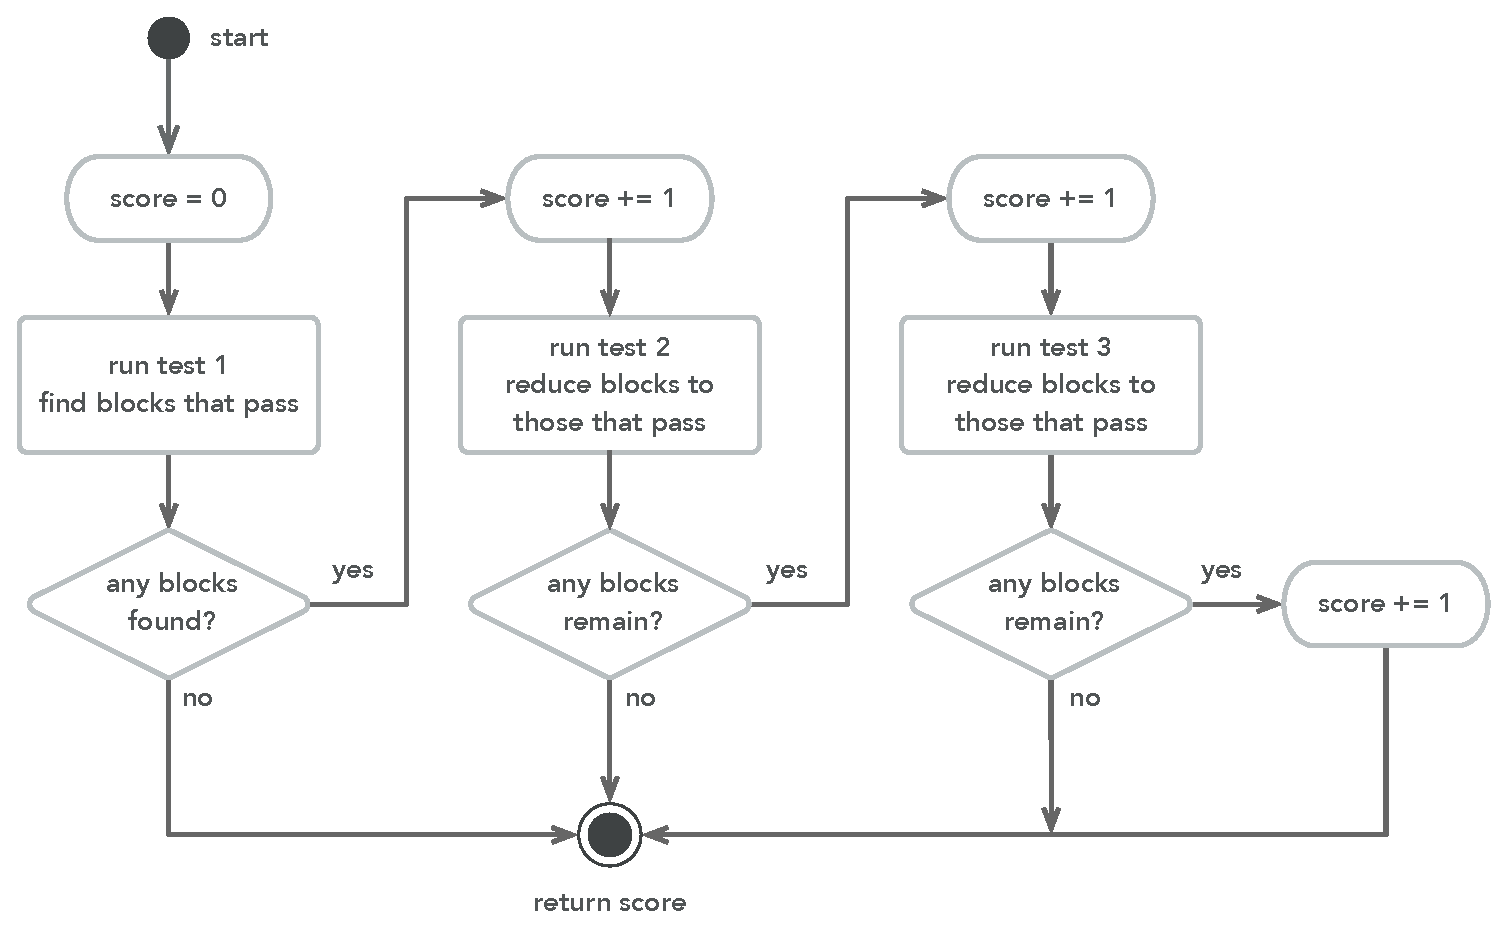
\includegraphics[width=\textwidth]{diagrams/particle-run3}
  \caption[Particle analysis test running algorithm]{Model of the algorithm for running particle analysis tests. This shows the three-test variant. There were also one- and two-test variants, that worked similarly. Test 1 must always be a ``find'' test that looks for individual blocks. Tests 2 and 3 must be ``in a'' tests, which investigate the parent blocks to assess nesting location. Available tests are listed in Table \ref{tab:particle-tests}.}
  \label{fig:particle-run3}
\end{figure}

The tests themselves come in two categories: ``find,'' which looked for certain blocks (the atom finder), and ``in a,'' which tested whether a block was ``in a'' specific parent block type. Additionally, there were helper routines of type ``this is'' which were used by the ``find'' and ``in a'' tests. The list of solution-defining particle tests is presented in Table \ref{tab:particle-tests}. In Figure \ref{fig:particle-run3}, test 1 must always be of the ``find'' type, and all subsequent tests must be of the ``in a'' type. 

\begin{table}
\begin{centering}
	\begin{tabular}{l l}
		Atom Finders (first test)			& Position Evaluators (subsequent tests) \\ \hline
		find number with value  			& in a division \\
		find text ``StopShaking'' 			& in a division position A	(dividend)	\\
		find text ``HowAreYou'' 			& in a division position B	(divisor)	\\
		find subtraction 					& in a subtraction 	\\
		find division 						& in a subtraction position A (minuend)	\\
		find multiplication					& in a subtraction position B (subtrahend)	\\
		find variable getter 				& in a multiplication	\\
		find procedure call 				& in a procedure call	\\
		find procedure definition			& in a procedure definition	\\
		find TextBox getText 				& in a set label text 	\\
		find Label setText					& in a textToSpeech speak	\\
		find event Button Click				& in a button click event	\\
		find event Accelerometer Shaking	& in an accelerometer shaking event 	\\
		find TextToSpeech Speak				& 	\\

	\end{tabular}
	\caption[Particle solution tests]{Tests that currently make up the solution particle definitions.}
	\label{tab:particle-tests}
\end{centering}
\end{table}

Implementation of these tests varied depending on what properties needed to be evaluated, but they all used helper tools to analyze the XML structure of the blocks workspace. Atom-finding tests were mostly a simple as checking each block for its designating property. Which property needed to be checked varied depending on the type of block, but they were all simple, constant-time reads. The position evaluators (``in a'' tests) were similarly simple, where each block's parent was looked up using the pre-rendered parent mapping structure, and the type of the parent was tested in the same fashion as the ``find'' tests. 

\label{sec:close-enough-text} %this belongs with the paragraph below wherever it ends up
Determining if a text string was equal to the solution's string was less straightforward, as there were many slightly different variations in phrasing that were all conceptually correct. An example was the ``stop shaking me'' text from the Debugging Activity. This string was fed into a text to speech engine to be spoken aloud, so any capitalization or punctuation combination were equally acceptable. Additionally, variations like ``please stop shaking me,'' ``stop shaking me now'' were also conceptually correct. A literal string compare would have regarded those falsely as incorrect. To find strings that were ``close enough'' to the exemplar, a Levenshtein edit distance was used \citep{levenshtein1966binary}. Specifically, what was used was a python implementation of an algorithm proposed by \citet{hyyro2001explaining}, which implemented the Levenshtein distance. To find the acceptable edit distances for ``good enough,'' all strings were collected from all of the activity projects in the database, along with their computed edit distance from their respective exemplar strings. The researchers sorted by edit distance value for each exemplar set, and chose a value which best delineated strings that were variations from those that were wrong. The values were different for the two exemplars: ``stop shaking me'' required an edit distance less than 9, and ``how are you'' required an edit distance less than 4. This process would need to be improved for teachers or curriculum developers to implement their own particle definitions. The method used by the researchers to reach their desired threshold values could be automated using hidden Markov Models, where ``close enough'' and ``not close enough'' examples provided by the user could automatically be assessed for a reasonable threshold value.


\section{The Classroom Console}
\label{sec:classroom-console}

\begin{figure}
  \centering
      \includegraphics{images/ch4-console-demo}
  \caption[Excerpt of the Classroom Console]{An excerpt of the Classroom Console visualization, showing three students.}
  \label{fig:console-demo}
\end{figure}


Based on the insights afforded by the particle analysis method, an orchestration technology was designed. Orchestration, as \citeauthor{dillenbourg2012design} described, ``refers to how a teacher manages in real-time multi-layered activities in a multi-constraints context" (\citeyear{dillenbourg2012design}). In the general case of App Inventor classrooms, teachers need to manage many levels of technology in addition to the difficult task of managing class-wide pedagogy, and the scaffolding of specific students as necessary. The orchestration technology developed here aims to support the activity of orchestrating \citep{tchounikine2013clarifying}.

The orchestration technology is referred to as the Classroom Console. An excerpt of the console is shown in Figure \ref{fig:console-demo}. This console, at a glance, gives teachers insight into the status of individual students and the class as a whole. Multiple dimensions of information are presented with visualization strategies that we believe are aggregated to a degree that makes it useful lightweight to use. The goals of the console are follows, for each student, it must display:

\begin{description}
\item [Current particle score] The primary display element is the student's current score. This is updated in real-time as they work.
\item [Time since score advanced] A ``timeout bar'' accompanies the score display, showing how much time has elapsed since the score has increased.
\item [Active or away] The timeout bar changes color to indicate whether the student is working actively or idle.
\end{description}

Additionally, the console must give the teacher a ``landscape view'' of the entire class. The visual score bars for each student are easily assessed as a group, so approximate progress of the entire class can be seen at a glance. If all the bars are low, then the class in general is either at the beginning, or may be in need of a class-wide clarification or hint. 

\subsection{Pre-Recorded Data}
This tool was a conceptual mockup. It did not work with live-collected data, but did operate on previously collected data from the study. The console as seen here is effectively a replay device, playing back real classroom data that were collected in real time. The data were genuine, and the timings expressed were the real-time observations of real students in their environments. This platform is ideal for design discussion. Connecting this concept to a live learning management environment is reserved for future work. 

\subsection{The Console in Detail}
A single student's display is annotated in Figure \ref{fig:console-single-annotated}. It shows the student's identifier, which could be their name (a), their current score on the problem from particle analysis (b), and a timeout bar (c). The timeout bar fills in one-minute intervals, starting with zero. The timeout bar also changes color to reflect when the student is no longer actively working, and has become idle. This ``away'' indicator can be seen in Figure \ref{fig:console-demo}, where the first two students are active and the third is away. The third student's idle bar is a lighter color.

A full classroom of 29 students is shown in Figure {fig:console-classroom}. There are many stories that can be deduced from this single moment. At the time of capture, many students had completed or near-completed the activity, indicated by the prevalence of tall blue bars. Students KermanshahCo, KobeSalamander, and PhoenixWeasel were examples of students who had completed the activity, and then became idle. Logically, at the conclusion of the activity these students became idle, as they had nothing left to do. They may have been elsewhere in the classroom, but were no longer engaging with App Inventor. Conversely, TaizhouSwallow, located in the lower-left corner of the Console, appeared to be having difficulty. This student is showing a low score, and has also been actively working with no forward progress for five minutes or more. Students with no indicators in the timeout bar, such as PointeCheetah and ShiheziBat in the middle row, had progressed their scores forward within the last minute. Every block in the timeout bar represented one minute of time, and a full bar of five blocks indicated five or more minutes without progress. 

\begin{figure}
  \centering
      \includegraphics{images/ch4-console-single-annotated}
  \caption[One student display, annotated]{One student's display from the Classroom Console. }
  \label{fig:console-single-annotated}
\end{figure}


\begin{figure}
  \centering
      \includegraphics[width=\textwidth]{images/ch4-console-class}
  \caption[Full classroom display of the Classroom Console]{A full classroom of 29 displayed in the Classroom Console.}
  \label{fig:console-classroom}
\end{figure}

